To describe the overall design of the Kite compiler, we will start by
breaking it down into general parts, where each part or module has a
specific task. Below we have a waterfall model including the main
parts of the compiler:

\begin{figure}[H]
  \label{fig:flow}
  \center
  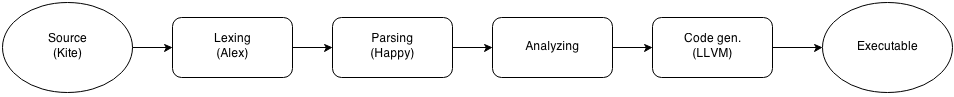
\includegraphics[scale=0.45]{images/flow.png}
  \caption{General flow of the Kite compiler}
\end{figure}

At first it can seem a little daunting, but when we get into the
purpose of each step, there will be a more obvious flow.

\subsection{Preprocessor}
The first thing the compiler does is preprocess the input, e.i. the
source code files, that it has been given. This is quite simply the
task of including all necessary files into one file. The files to be
included are declared in the top of the file.

\begin{figure}[H]
  \label{fig:preprocessor}
  \center
  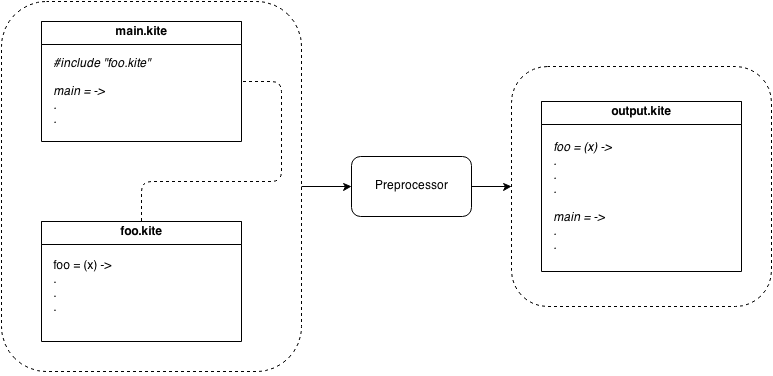
\includegraphics[scale=0.45]{images/preprocessor.png}
  \caption{Input and output of the Preprocessor}
\end{figure}

The nature of the preprocessor is quite simple, as the only task it
simple textual substitution.


\subsection{Lexical analysis}
The lexical analyzer, or just \emph{lexer}, is a central part of most
compilers. It has the important task of processing some input and
converting it to known, referencable tokens. This process is commonly
known as \emph{tokenization}.

Most lexers are quite simple, as they simply make tokens by matching the input with regular languages and classify the substrings according to these. Thus lexers do not perform any complex tasks - this is reserved for the parser and analyzer, which we will describe in the following.


\subsection{Parser}
The parser takes the list of tokens from the lexer and based on a
language grammar, it builds a corresponding data structure, namely the
parse tree. In the process it checks that that the input is
syntactically correct. Therefore, this process is also called syntactic
analysis.

In the cases know to us (Yacc, Happy, ANTLR), parser-generators make use of \emph{Context-Free Grammars} (CFG), and thus we have to define our desired syntax as a CFG.

The parser should rule out code containing syntactical errors, especially typos, which are likely to occur without a good IDE\footnote{IDE is short for Integrated Development Environment, which, among other features, often has good auto-completion, thus making typos much less likely.}.


\subsection{Desugar}
In order to make the language more convenient to write, we have made syntactic sugar and will introduce a desugaring module. This will take specific syntactic constructs and convert them into their more basic elements.


\subsection{Analyzer}
Tha analyzer is the first component of the compiler's back-end (or middle-end, to avoid confusion with code-generation). It will traverse the parse tree and perform \emph{typechecking} and look for calls to undefined functions. The analyser should spot almost all remaining incorrect code. Thus the output should be able to be executed without errors due to incorrect types, typos or the usage of undeclared variables.

The analyzer cannot, however, determine whether a program will yield the expected results or even if it will ever terminate.


\subsection{Optimizer}
The optimizer module takes the AST and transforms it in such a way that the program is faster or smaller, but the functionality is the same. This is described in more detail in section \ref{sec:impl-optimizer}.


\subsection{Code generation}
The code generator will take the AST outputted from the parser, and emit code for a specified target language. Currently Kite only supports one code generation backend namely for JavaScript, but the module is structured in such a way that allows easy integration with new code generation modules.

\textbf{LLVM as backend:} The LLVM compiler
infrastructure\footnote{LLVM Project \url{http://llvm.org/}} will allow
for low level binary machine code generation. The LLVM infrastructure
will take a representation of the parse tree and emit a LLVM
intermediate representation (IR) which can be used for code
generation. Since LLVM is strong statically typed, a modified variant
of Kites parse tree is needed. The LLVM infrastructure will also provide
optimization passes for a given LLVM IR.

\textbf{JavaScript as backend:} As an alternative, a JavaScript emitter
can be implemented and used as backend. Since JavaScript is untyped,
Kite can rely on the typechecker and emit JavaScript. The emitted
JavaScript should not contain type errors, as the analyzer will
catch type errors. The emitted JavaScript will run on the
Node.js platform\footnote{ The Node.js platform \url{nodejs.org}}.
Node.js makes use of the Google V8 JavaScript engine \footnote{Google
  V8 engine \url{http://code.google.com/p/v8/}} which compiles JavaScript to
native machine code. The result is faster and more optimized
JavaScript execution.

%%% Local Variables:
%%% mode: latex
%%% TeX-master: "../report"
%%% End:
